\section{Signal Processing}

The signal processing phase is crucial in converting the raw audio input into a format suitable for beat detection. This section explains the preprocessing steps, such as filtering and energy calculation, and justifies the selection of signal processing techniques.

\subsection{Preprocessing the Audio File}

\subsubsection{Filtering}

The preprocessing process starts by applying a low-pass Butterworth filter to reduce high-frequency components that are not relevant to beat detection. This filter is preferred due to its flat passband, which ensures minimal distortion of relevant frequencies.

\begin{itemize}
    \item \textbf{Cutoff Frequency:} The \texttt{CUTOFF\_FREQUENCY}, set to 300 Hz, delineates the frequency above which signals are attenuated, chosen to retain fundamental rhythmic components while simplifying the beat detection.
    \item \textbf{Filter Order:} The \texttt{FILTER\_ORDER\_LIMIT} is configured at 5, balancing the need for a sharp frequency cutoff against minimizing phase distortions.
\end{itemize}

\subsubsection{Energy Signal Calculation}

After filtering, the energy of the signal is calculated by applying short, overlapping windows. This transformation emphasizes rhythmic patterns.

\begin{itemize}
    \item \textbf{Windowing:} The signal is segmented into windows, within which the amplitude values are squared and summed to yield the energy.
    \item \textbf{Smoothing:} The energy signal is smoothed (using a window specified by \texttt{SMOOTHING\_WINDOW\_DURATION}, defaulting to 0.01 seconds) to reduce fluctuations and emphasize beats.
\end{itemize}

\subsection{Visualization of Energy Calculation}

The graph below illustrates the process of energy calculation and smoothing. It plots normalized energy against time, represented in samples per thousand. The blue line represents the original energy signal, which shows the raw energy levels derived from the audio file. The red line represents the smoothed energy signal, which is the result of applying a moving average filter to the original energy.

\begin{figure}[H]
    \centering
    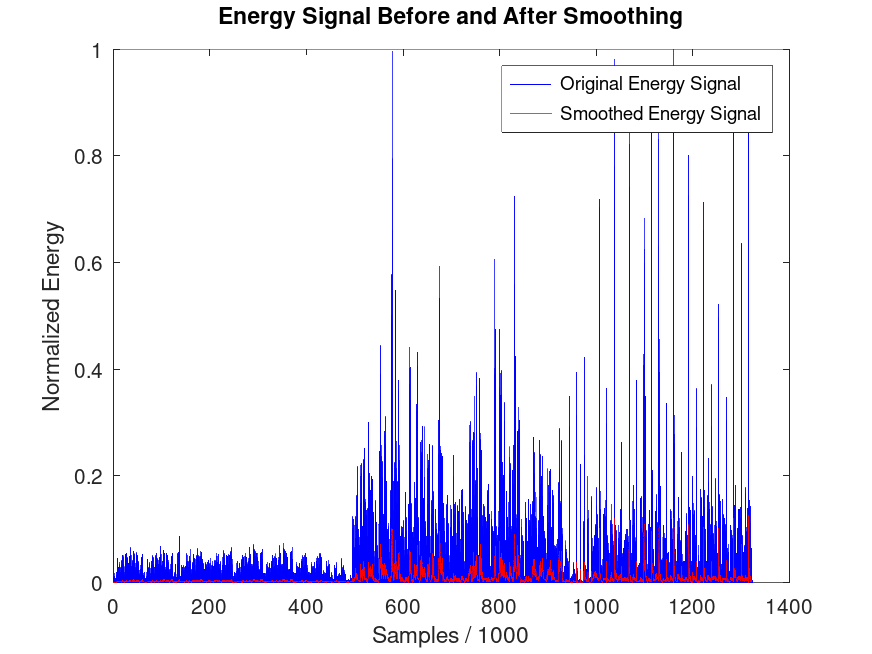
\includegraphics[width=0.8\textwidth]{energy.png}
    \caption{Normalized energy of the audio signal with original and smoothed energy.}
\end{figure}

\subsubsection{Effect of Moving Average Smoothing}

The original energy signal is smoothed using the moving average technique to reduce short-term fluctuations and emphasize underlying trends. This is done by averaging the energy values within a specified window (\texttt{SMOOTHING\_WINDOW\_DURATION}) that moves across the signal. Each point in the smoothed signal represents the average energy of the surrounding points within the window, effectively minimizing the impact of transient spikes or drops in energy.

The reason for smoothing the energy signal is to emphasize rhythmic patterns, which are crucial for precise beat detection. The moving average filter helps to identify significant peaks that correspond to the music's rhythm by reducing noise and highlighting sustained energy levels that indicate beats. This approach ensures that the subsequent beat detection process focuses on genuine rhythmic content rather than being misled by momentary energy changes.

\subsection{Conclusion}

The signal processing phase, which includes filtering and energy signal calculation, is crucial in converting raw audio into a format suitable for beat detection. The combination of low-pass filtering and energy smoothing prepares the audio signal by highlighting rhythmically significant patterns. The graph illustrates how the moving average filter smooths the energy signal, making rhythmic peaks more prominent and thus facilitating more reliable beat detection. Through these carefully selected processing steps, the project establishes a solid foundation for accurately detecting beats across various musical styles, demonstrating its effectiveness as an advanced beat detection system.
